\documentclass[a4j,titlepage]{jsarticle}

\usepackage[dvipdfmx]{graphicx,xcolor}
\usepackage[top=20truemm,left=25truemm,right=25truemm]{geometry}
\usepackage{amsmath}
\usepackage{here}
\usepackage{plistings}
\usepackage{tikz}
\usepackage[framemethod=tikz]{mdframed}

\renewcommand{\lstlistingname}{リスト}

\newcommand{\chuo}[1]{\multicolumn{1}{|c|}{#1}}
\newcommand{\inpt}[1]{\underline{#1}\,\setlength{\fboxsep}{1pt}\fbox{\small ↓}}

\lstdefinestyle{yaml}{
    language=,
    basicstyle=\small\ttfamily,
    keywordstyle=\color[HTML]{0000E0},
    stringstyle=\color[HTML]{A31515},
    commentstyle=\upshape\color[HTML]{008000},
    frame=trbl,
    framesep=5pt,
    columns=[l]{fullflexible},
    numbers=left,
    xleftmargin=3zw,
    lineskip=-0.2ex,
    breaklines=true,
    showstringspaces=false,
    tabsize=4,
    keepspaces=true
}

\lstdefinestyle{sql}{
    language=sql,
    basicstyle=\small\ttfamily,
    keywordstyle=\color[HTML]{0000E0},
    stringstyle=\color[HTML]{A31515},
    commentstyle=\upshape\color[HTML]{008000},
    frame=trbl,
    framesep=5pt,
    columns=[l]{fullflexible},
    numbers=left,
    xleftmargin=3zw,
    lineskip=-0.2ex,
    breaklines=true,
    showstringspaces=false,
    tabsize=4,
    keepspaces=true
}

\lstdefinestyle{ruby}{
    language=ruby,
    basicstyle=\small\ttfamily,
    keywordstyle=\color[HTML]{0000E0},
    stringstyle=\color[HTML]{A31515},
    commentstyle=\upshape\color[HTML]{008000},
    frame=trbl,
    framesep=5pt,
    columns=[l]{fullflexible},
    numbers=left,
    xleftmargin=3zw,
    lineskip=-0.2ex,
    breaklines=true,
    showstringspaces=false,
    tabsize=4,
    keepspaces=true
}

\lstdefinestyle{html}{
    language=html,
    basicstyle=\small\ttfamily,
    keywordstyle=\color[HTML]{0000E0},
    stringstyle=\color[HTML]{A31515},
    commentstyle=\upshape\color[HTML]{008000},
    frame=trbl,
    framesep=5pt,
    columns=[l]{fullflexible},
    numbers=left,
    xleftmargin=3zw,
    lineskip=-0.2ex,
    breaklines=true,
    showstringspaces=false,
    tabsize=4,
    keepspaces=true
}

\lstdefinestyle{js}{
    language=java,
    basicstyle=\small\ttfamily,
    keywordstyle=\color[HTML]{0000E0},
    stringstyle=\color[HTML]{A31515},
    commentstyle=\upshape\color[HTML]{008000},
    frame=trbl,
    framesep=5pt,
    columns=[l]{fullflexible},
    numbers=left,
    xleftmargin=3zw,
    lineskip=-0.2ex,
    breaklines=true,
    showstringspaces=false,
    tabsize=4,
    keepspaces=true
}

\lstdefinestyle{css}{
    language=,
    basicstyle=\small\ttfamily,
    keywordstyle=\color[HTML]{0000E0},
    stringstyle=\color[HTML]{A31515},
    commentstyle=\upshape\color[HTML]{008000},
    frame=trbl,
    framesep=5pt,
    columns=[l]{fullflexible},
    numbers=left,
    xleftmargin=3zw,
    lineskip=-0.2ex,
    breaklines=true,
    showstringspaces=false,
    tabsize=4,
    keepspaces=true
}

\lstdefinestyle{text}{
    language=,
    basicstyle=\ttfamily,
    frame=trbl,
    framesep=5pt,
    columns=[l]{fullflexible},
    xleftmargin=3zw,
    lineskip=-0.2ex,
    showstringspaces=false,
    tabsize=4,
    keepspaces=true
}

\mdfsetup{
    skipabove=5pt,
    innertopmargin=10pt,
    innerbottommargin=10pt,
    roundcorner=10pt,
    font=\ttfamily
}


\begin{document}


\begin{titlepage}
  \title{\huge{ネットワークプログラミングI} \\ \LARGE{---Webアプリケーションの作成---}}
	\author{学籍番号:16426 \\ 4年 電子情報工学科 23番 \\ 福澤 大地}
	\date{提出日 : 2020年2月17日}
  \maketitle
\end{titlepage}


\section{目的}
RubyでWebアプリケーションを作成することで、講義で身につけたサーバーサイドプログラミング、
フロントエンドプログラミング、データベースなどの総合的な技術を強化する。

また、外部者からの攻撃などを想定し、それに対する対策を施すことで、セキュリティに関する知識を身に付ける。


\section{開発環境}
アプリケーションを開発するにあたって、仮想化ソフトフェアであるVurtualBoxを用いて仮想環境を構築した。
ホストOSの環境を表\ref{tb:kan}, 仮想環境を表\ref{tb:virtual}に示す。

\begin{table}[H]
  \centering
  \caption{ホストOSの環境}
  \label{tb:kan}

  \begin{tabular}{|l|l|}
    \hline
    CPU & Intel Core i5-7400 @ 3.0GHz \\ \hline
    メモリ & 8GB \\ \hline
    OS & Microsoft Windows 10 Home \\ \hline
    システム & 64bit \\ \hline
    Webブラウザ & Google Chrome 77.0.3865.120 \\ \hline
  \end{tabular}
\end{table}

\begin{table}[H]
  \centering
  \caption{仮想環境}
  \label{tb:virtual}

  \begin{tabular}{|l|l|}
    \hline
    仮想化ソフトフェア & Oracle VirtualBox 6.0.12 \\ \hline
    割り当てメモリ & 2GB \\ \hline
    OS & CentOS 7.6 \\ \hline
    システム & 64bit \\ \hline
    開発言語 & Ruby 2.6.2 \\ \hline
    データベース & SQLite3 3.7.17 \\ \hline
  \end{tabular}
\end{table}

今回は仮想環境上でWebアプリケーションを実行し、ホストOSのWebブラウザからアクセスする。
つまり、ホストOSと仮想環境を別々の2つのコンピュータと捉えて通信を行う。
URLには次のように入力する。

\begin{mdframed}
  http://localhost:9998/
\end{mdframed}

\texttt{localhost}というのはループバックアドレスであり、自分自身にパケットを返す。
末尾の\texttt{:9998}で9998番ポートでパケットを受け取ることを指定している。


\section{Gemパッケージのインストール}
Rubyでアプリケーションを作るにあたって、まずは必要なGemパッケージをインストールしておく必要がある。
GemパッケージとはRubyで使われるライブラリのことである。
Gemパッケージをインストールするために、アプリケーションフォルダにパッケージを整えてくれるソフトウェア (Bundler)を使用する。
アプリケーションフォルダに移動し、次のように入力して実行する。

\begin{mdframed}
  bundle init
\end{mdframed}

実行すると自動的に作成されるGemfileというファイルを、リスト\ref{gem}のように書き換える。
Gemfileとは、Bundlerの設定ファイルである。

\lstinputlisting[style=ruby,caption=Gemfile,label=gem]{../Gemfile}

Gemfileで指定したパッケージの概要について次に示す。

\begin{itemize}
  \item{sinatra ... WebアプリケーションフレームワークであるSinatraを使うためのライブラリ}
  \item{sqlite3 ... データベース管理システムであるSQLite3を使うためのライブラリ}
  \item{activerecord ... Rubyでデータベースを扱うためのライブラリ}
\end{itemize}

最後に次のように入力して。必要なパッケージをインストールする。

\begin{mdframed}
  bundle install --path vendor/bundle
\end{mdframed}

vendorというフォルダが作成され、このフォルダの中にパッケージがインストールされる。
実際にインストールされたパッケージは、Gemfileと同じディレクトリのGemfile.lockに記述されている。


\section{データベースの設計}
今回作成した掲示板のWebアプリケーションでは、書き込みを格納するためにデータベースを使用する。
データベース管理システムはSQLite3である。
テーブルを作成するにはプロンプトから一行ずつコマンドを打ち込んでつくるという方法もあるが、
テーブルに変更を加えたり、初期化したりするときにいちいち最初から打ち込むのは面倒である。
そのため、リスト\ref{dbinit}のようなSQL文を記述したファイルを作成しておくと便利である。

\lstinputlisting[style=sql,caption=bbs.sql,label=dbinit]{../bbs.sql}

これをbbs.sqlとして保存し、次のように打ち込むとbbs.dbが作成される。

\begin{mdframed}
  sqlite3 bbs.db \verb|<| bbs.sq3
\end{mdframed}

投稿を格納するテーブルpostsの設定を表\ref{writings}、
アカウント情報を格納するテーブルaccountsの設定を表\ref{accounts}に示す。

\begin{table}[h]
  \centering
  \caption{postsテーブルの概要}
  \label{writings}
  \begin{tabular}{|l|l|l|}
    \hline
    \chuo{フィールド名} & \chuo{型} & \chuo{内容} \\ \hline \hline
    number & INTEGER & 投稿番号 \\ \hline
    exist  & INTEGER & 投稿が存在してるか (削除されていないか) \\ \hline
    kind   & INTEGER & 投稿の種類 (0:テキスト, 1:イラスト) \\ \hline
    time   & CHAR(24) & 投稿した時刻     \\ \hline
    userid & VARCHAR(64) & 投稿者のユーザーID \\ \hline
    text   & VARCHAR(1024) & 投稿内容   \\ \hline
    origin & INTEGER & 元にしたイラストの投稿番号  \\ \hline
  \end{tabular}
\end{table}

\begin{table}[h]
  \centering
  \caption{accountsテーブルの概要}
  \label{accounts}
  \begin{tabular}{|l|l|l|}
    \hline
    \chuo{フィールド名} & \chuo{型} & \chuo{内容} \\ \hline \hline
    userid & INTEGER    & ユーザーID \\ \hline
    salt & CHAR(32)   & ハッシュ化の際に用いるソルト     \\ \hline
    hashed & CHAR(32) & 認証用のハッシュ値     \\ \hline
    name & VARCHAR(64)      & アカウント名     \\ \hline
  \end{tabular}
\end{table}


\section{YAMLについて}
YAML (YAML Ain't a Markup Language)はXMLのように構造化されたデータを、XMLよりも人間に読み書きしやすい形にしたものである。
アプリケーションでbbs.dbを扱うために、ソースコード\ref{yml}ようにdatabase.ymlを作成する。
プログラム内でこのファイルを読み込むと、指定したデータベースを操作できるようになる。

\lstinputlisting[style=yaml,caption=database.yml,label=yml]{../database.yml}


\section{ActiveRecordについて}
ActiveRecordはデータベースのレコードをオブジェクト指向言語のオブジェクトに対応させるライブラリである。
そうすることでオブジェクト指向言語でオブジェクトを操作すると、
内部的にデータベース管理システムのコマンドを発行し、
適切にデータベースを操作して結果を返してくれる。
SQLite3やMySQLなどのデータベース管理システムの違いをActiveRecordが吸収することで、
様々なデータベースをオブジェクト指向言語のオブジェクトへ対応させている。


\section{Webアプリケーションの構造}
今回作成したアプリケーションでは、処理部分と表示部分を分離させている。
処理本体はRubyで記述するが、表示はHTMLコードの中にRubyのコードを埋め込むことができるEmbedded Rubyで記述する。
Embedded Rubyは、表\ref{erb}に示すルールでRubyのコードを埋め込むことができる。

\begin{table}[H]
  \centering
  \caption{erbのルール}
  \label{erb}
  \begin{tabular}{|l|l|}
    \hline
    \chuo{記述} & \chuo{意味} \\ \hline \hline
    {\tt\verb|<%= code %>|}    & 囲まれた部分を実行して結果を埋め込む。         \\ \hline
    {\tt\verb|<% code %>|}     &  囲まれた部分を実行するが、結果は埋め込まない。 \\ \hline
    {\tt\verb|<%# comment %>|} &  囲まれた部分をコメントアウトする。            \\ \hline
  \end{tabular}
\end{table}

見た目を表すEmbedded Rubyのファイルは、viewsディレクトリの中に作成する。
アプリケーションフォルダのディレクトリ構造を図\ref{dir}に示す。

\begin{figure}[H]
\centering
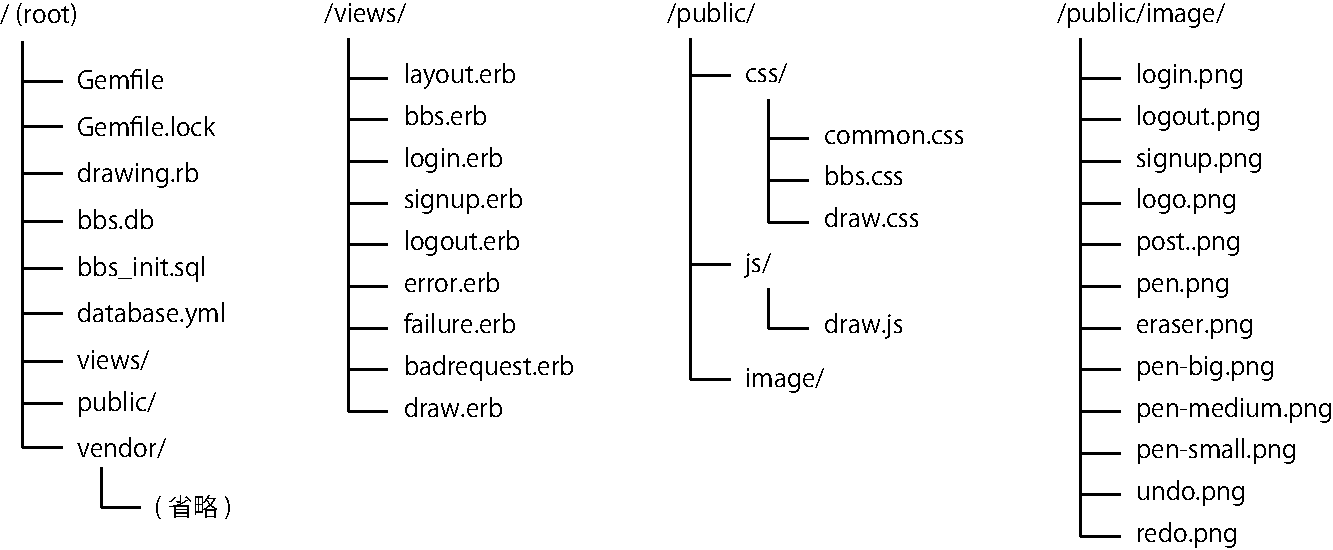
\includegraphics[width=14cm]{file.pdf}
\caption{ディレクトリ構造}
\label{dir}
\end{figure}


\section{プログラムリスト}
図\ref{dir}で示した各プログラムのソースコードを、リスト\ref{drawing}-\ref{drawjs}に示す。

\lstinputlisting[style=ruby,caption=drawing.rb,label=drawing]{../drawing.rb}

\lstinputlisting[style=html,caption=layout.erb,label=layout]{../views/layout.erb}

\lstinputlisting[style=html,caption=bbs.erb,label=bbs]{../views/bbs.erb}

\lstinputlisting[style=html,caption=login.erb,label=login]{../views/login.erb}

\lstinputlisting[style=html,caption=signup.erb,label=signup]{../views/signup.erb}

\lstinputlisting[style=html,caption=logout.erb,label=logout]{../views/logout.erb}

\lstinputlisting[style=html,caption=error.erb,label=error]{../views/error.erb}

\lstinputlisting[style=html,caption=failure.erb,label=failure]{../views/failure.erb}

\lstinputlisting[style=html,caption=badrequest.erb,label=badrequest]{../views/badrequest.erb}

\lstinputlisting[style=html,caption=draw.erb,label=draw]{../views/draw.erb}

\lstinputlisting[style=css,caption=common.css,label=commoncss]{../public/css/common.css}

\lstinputlisting[style=css,caption=bbs.css,label=bbscss]{../public/css/bbs.css}

\lstinputlisting[style=css,caption=draw.css,label=drawcss]{../public/css/draw.css}

\lstinputlisting[style=js,caption=draw.js,label=drawjs]{../public/js/draw.js}


\section{画像}
プログラム中で用いられる画像を図\ref{fig:logo}--\ref{fig:redo}に示す。

\begin{figure}[H]
  \centering
  
\includegraphics[width=6cm]{../public/image/logo.png}
  \caption{logo.png}
  \label{fig:logo}
\end{figure}

\begin{figure}[H]
  \centering
  
\includegraphics[width=4cm]{../public/image/login.png}
  \caption{login.png}
  \label{fig:login}
\end{figure}

\begin{figure}[H]
  \centering
  
\includegraphics[width=4cm]{../public/image/logout.png}
  \caption{logout.png}
  \label{fig:logout}
\end{figure}

\begin{figure}[H]
  \centering
  
\includegraphics[width=4cm]{../public/image/signup.png}
  \caption{signup.png}
  \label{fig:signup}
\end{figure}

\begin{figure}[H]
  \centering
  
\includegraphics[width=4cm]{../public/image/post.png}
  \caption{post.png}
  \label{fig:post}
\end{figure}

\begin{figure}[H]
  \centering
  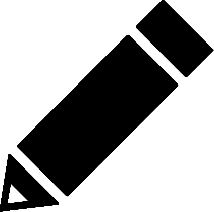
\includegraphics[width=3cm]{../public/image/pen.png}
  \caption{pen.png}
  \label{fig:pen}
\end{figure}

\begin{figure}[H]
  \centering
  
\includegraphics[width=3cm]{../public/image/eraser.png}
  \caption{eraser.png}
  \label{fig:eraser}
\end{figure}

\begin{figure}[H]
  \centering
  
\includegraphics[width=3cm]{../public/image/pen-big.png}
  \caption{pen--big.png}
  \label{fig:penbig}
\end{figure}

\begin{figure}[H]
  \centering
  
\includegraphics[width=3cm]{../public/image/pen-medium.png}
  \caption{pen--medium.png}
  \label{fig:penmedium}
\end{figure}

\begin{figure}[H]
  \centering
  
\includegraphics[width=3cm]{../public/image/pen-small.png}
  \caption{pen--small.png}
  \label{fig:pensmall}
\end{figure}

\begin{figure}[H]
  \centering
  
\includegraphics[width=3cm]{../public/image/undo.png}
  \caption{undo.png}
  \label{fig:undo}
\end{figure}

\begin{figure}[H]
  \centering
  
\includegraphics[width=3cm]{../public/image/redo.png}
  \caption{redo.png}
  \label{fig:redo}
\end{figure}


\section{実装機能}
\subsection{アカウント登録}
アカウントを新規登録するためのフォームを図\ref{signup}に示す。
ユーザー名、ユーザーID、パスワードを入力し、新規登録ボタンを押すと、/registにPOSTし、drawing.rbの142行目でキャッチする。
ユーザーIDが既に存在していたり、確認用のパスワードが異なっていればエラーページを表示し、正常な入力ならaccountsテーブルにアカウントを登録する。
生のパスワードにランダムな文字列であるソルトを連結した文字列のハッシュ値を記録しておくことで、生のパスワードが保存されることはないので、テーブルの内容が盗み見られても安全である。

\begin{figure}[H]
  \centering
  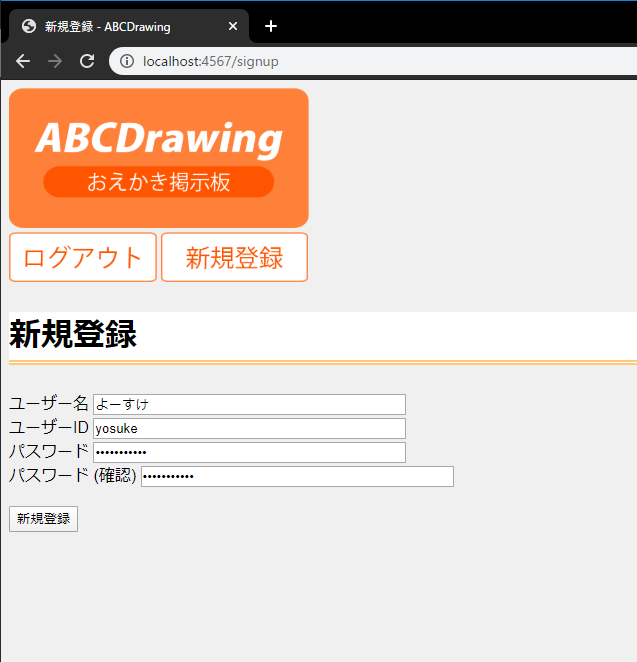
\includegraphics[width=10cm]{signup.png}
  \caption{新規登録フォーム}
  \label{signup}
\end{figure}

\subsection{ログイン}
ログインをするためのフォームを図\ref{login}に示す。
ユーザーIDとパスワードを入力し新規登録ボタンを押すと、/authにPOSTし、drawing.rbの178行目でキャッチする。
パスワードにソルトを連結した文字列のハッシュ値と、新規登録の際に記録したハッシュ値を比較し、一致していたらCookieにログイン中であることを記録する。
ユーザーIDが存在していなかったり、パスワードが間違っていたら、図\ref{failed}のページを表示する。

\begin{figure}[H]
  \centering
  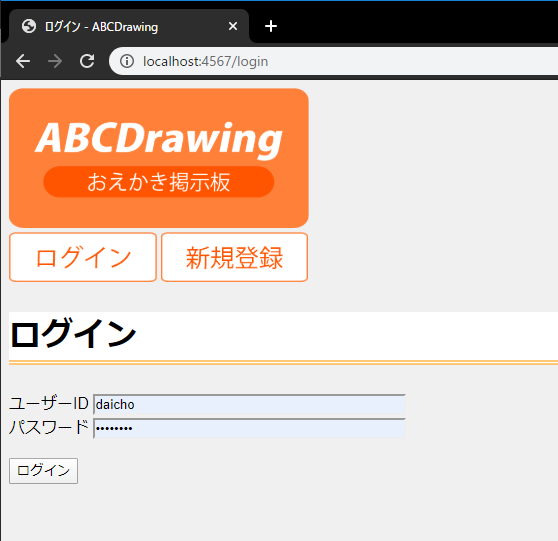
\includegraphics[width=10cm]{login.png}
  \caption{ログインフォーム}
  \label{login}
\end{figure}

\begin{figure}[H]
  \centering
  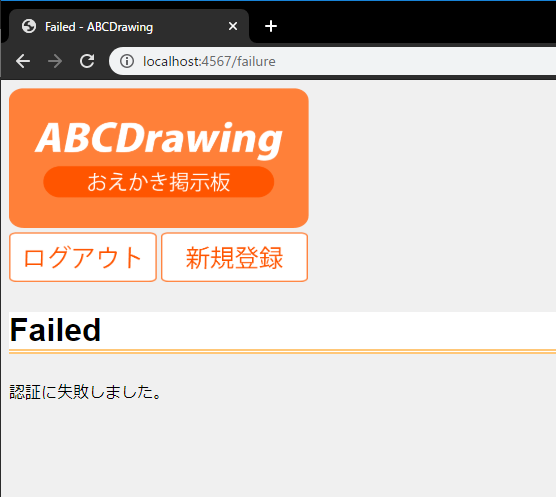
\includegraphics[width=10cm]{failed.png}
  \caption{ログイン失敗}
  \label{failed}
\end{figure}

\subsection{ログアウト}
ログアウトボタンを押した場合は、Cookieの内容を消去する。
そうすることで、ログイン中の情報が消えるため、ログアウトできる。

\subsection{テキスト投稿}
図\ref{f1}のように、名前とテキストを入力し、``書き込み''ボタンを押下すると掲示板にその内容が書き込まれる。
書き込まれた様子を図\ref{f2}に示す。
図\ref{f2}を見ると、投稿内容の他に、投稿番号、書き込んだユーザーの名前、日時も記録されていることが分かる。

\begin{figure}[H]
  \centering
  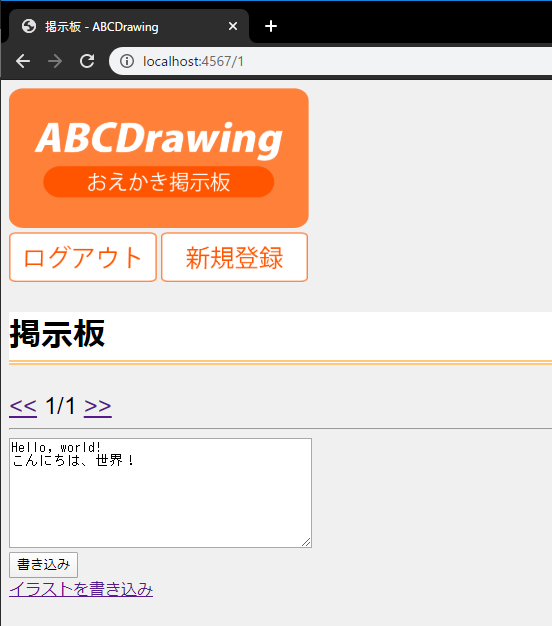
\includegraphics[width=10cm]{bbs02.png}
  \caption{投稿前の様子}
  \label{f1}
\end{figure}

\begin{figure}[H]
  \centering
  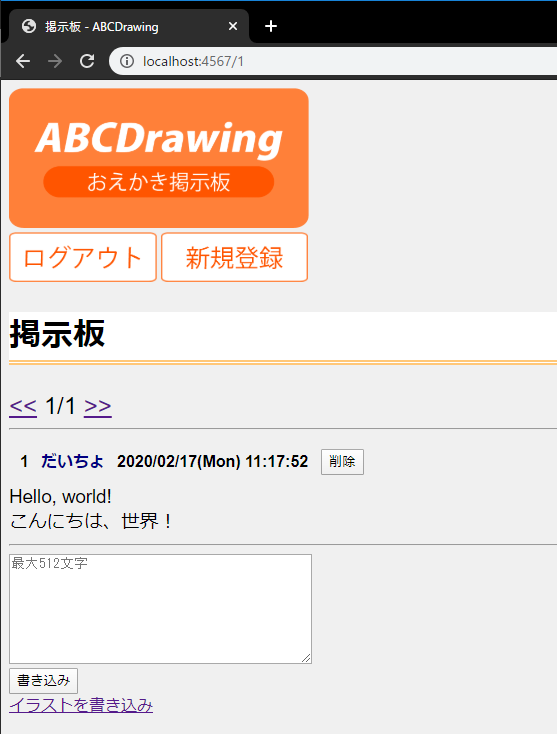
\includegraphics[width=10cm]{bbs03.png}
  \caption{投稿後の様子}
  \label{f2}
\end{figure}

入力フォームのHTMLは、bbs.erbの68行目以降に実装されている。
ボタンを押すと/new\_textにPOSTし、それをサーバーサイドのプログラムdrawing.rbの54行目でキャッチする。
ここでは、投稿番号、日時、投稿内容、ユーザーIDを取得し、ActiveRecordを介してデータベースに投稿を記録している。

\subsection{投稿の削除}
ここで、別のアカウントでログインし、投稿を行った状態を図\ref{f0}に示す。
図\ref{f0}を見ると、2つ目の投稿の横にだけ``削除''ボタンがあるのが分かる。
これは、自身が行った投稿の横にのみ表示される。
このボタンを押すと投稿が削除され、図\ref{del}のように、投稿内容が表示されなくなる。

``削除''ボタンを押すと/deleteにリダイレクトされるように設定されており、このときbbs.rbの80行目以降が実行される。
当該の投稿をデータベースから検索し、existカラムの値を0にすることで、投稿が削除される。

\begin{figure}[H]
  \centering
  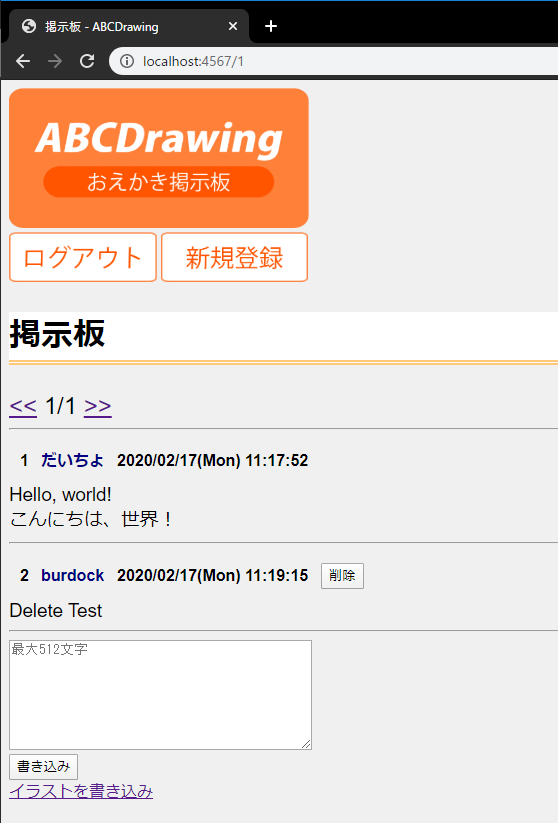
\includegraphics[width=10cm]{bbs04.png}
  \caption{削除前の状態}
  \label{f0}
\end{figure}

\begin{figure}[H]
  \centering
  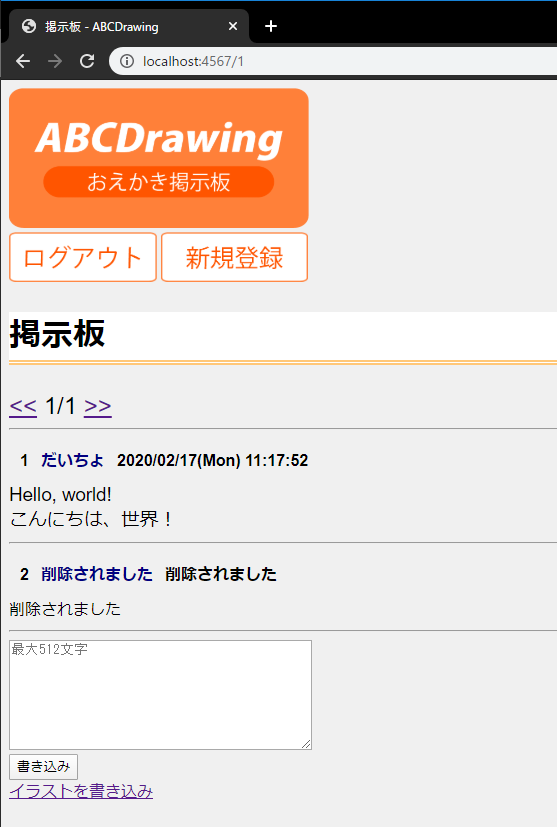
\includegraphics[width=10cm]{bbs05.png}
  \caption{削除後の状態}
  \label{del}
\end{figure}

\subsection{サニタイズと改行}
\verb|<|や\verb|'|などの特殊な文字も入力できるように入力内容に対してサニタイズを行った。
サニタイズをすることで、HTMLタグを不正に実行される脆弱性を予防する効果もある。
また今回は、改行コードをHTMLタグ{\tt\verb|<br>|}に変換することで改行の入力を可能にした。

特殊な文字と改行を混じえた投稿の様子を図\ref{f3}に示す。
図\ref{f3}を見ると、各記号が正しく投稿されており、改行もされていることが分かる。

\begin{figure}[H]
  \centering
  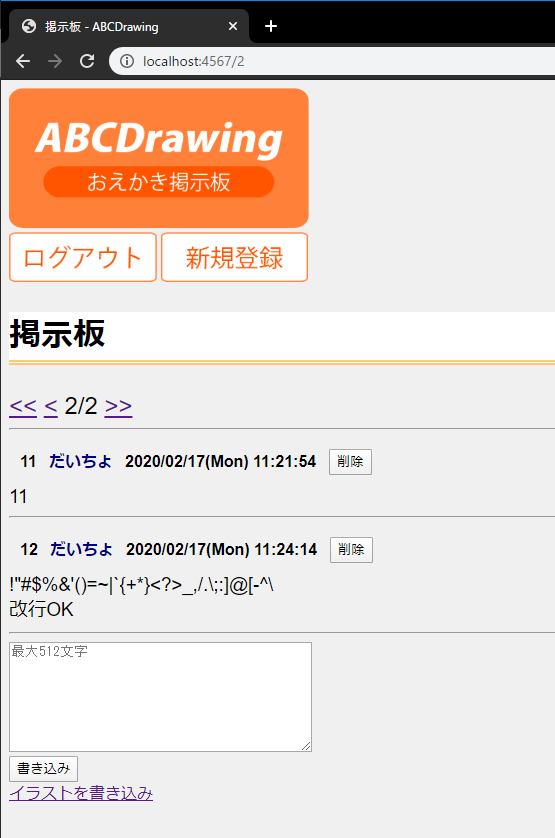
\includegraphics[width=10cm]{bbs10.png}
  \caption{サニタイズと改行}
  \label{f3}
\end{figure}

\subsection{入力文字数制限}
bbs.erbの72, 73行目を見ると、textarea要素にrequired, maxlength属性が付与されていることが分かる。
これにより、文字を入力していなくても文字数が多すぎても投稿出来ないようになっている。
図\ref{f4}は、文字を入力せずに投稿ボタンを押した時の挙動である。

\begin{figure}[H]
  \centering
  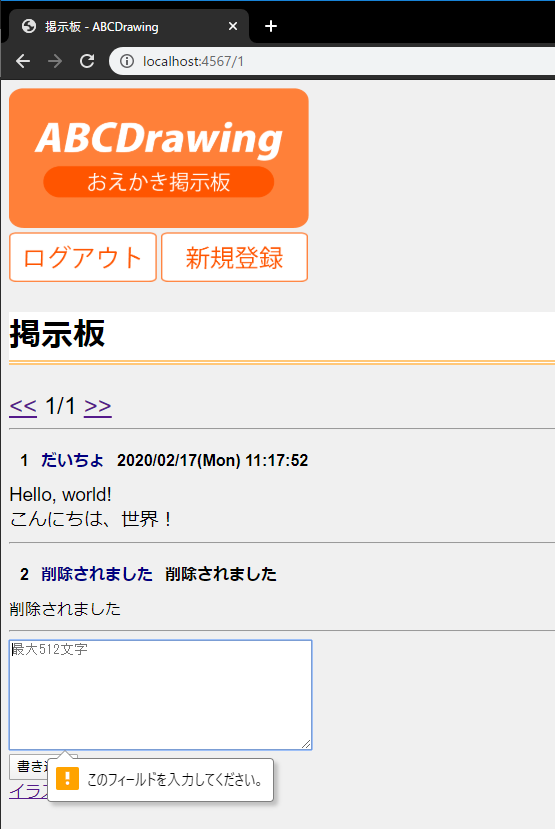
\includegraphics[width=10cm]{bbs06.png}
  \caption{入力必須フォーム}
  \label{f4}
\end{figure}

\subsection{イラスト投稿}
テキストの他に、自分で描いたイラストを投稿できる機能を実装した。
イラストを描くフォームを図\ref{draw}に示す。
消しゴム、ペンの太さを指定できる他、ペンの色指定とUndo/Redoをできるようにした。

\begin{figure}[H]
  \centering
  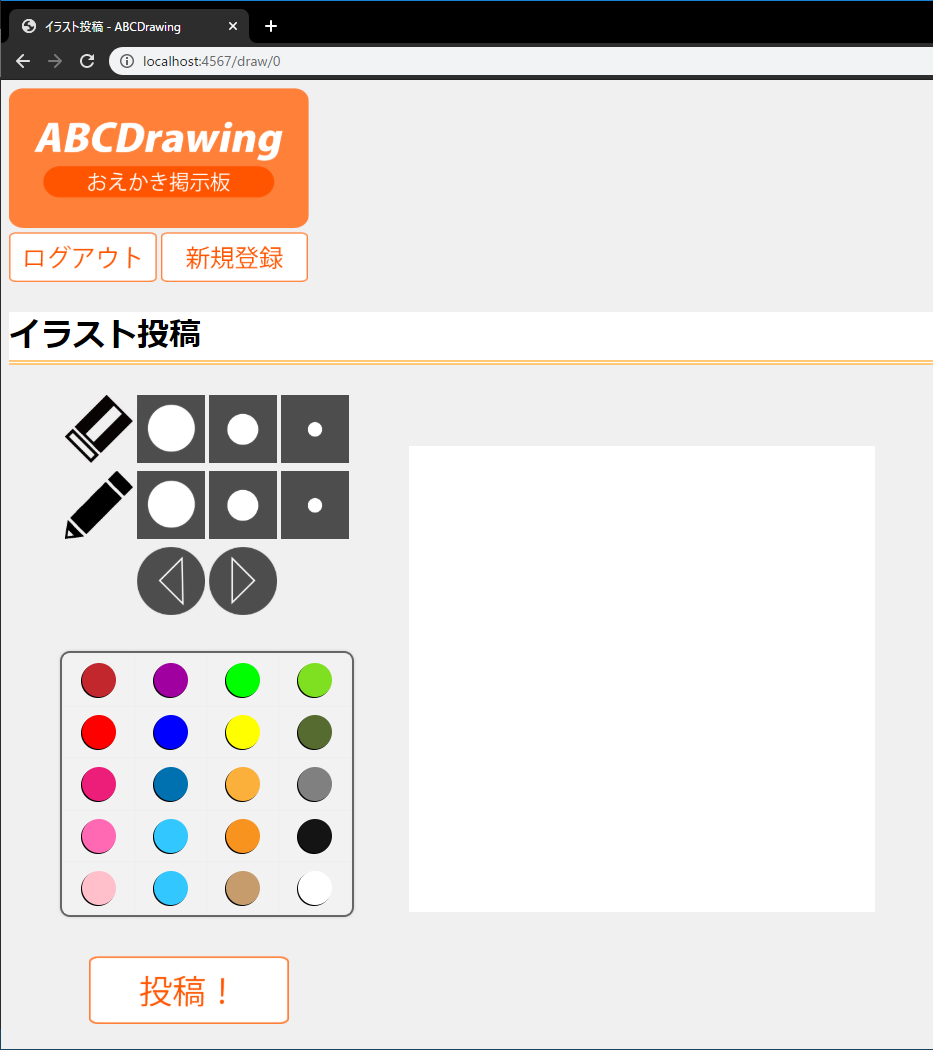
\includegraphics[width=14cm]{draw.png}
  \caption{おえかきフォーム}
  \label{draw}
\end{figure}

イラストを描いた様子を図\ref{drawdaruma}に示す。
この状態で投稿ボタンを押すと、図\ref{drawpost}のように、描いたイラストが投稿できる。

\begin{figure}[H]
  \centering
  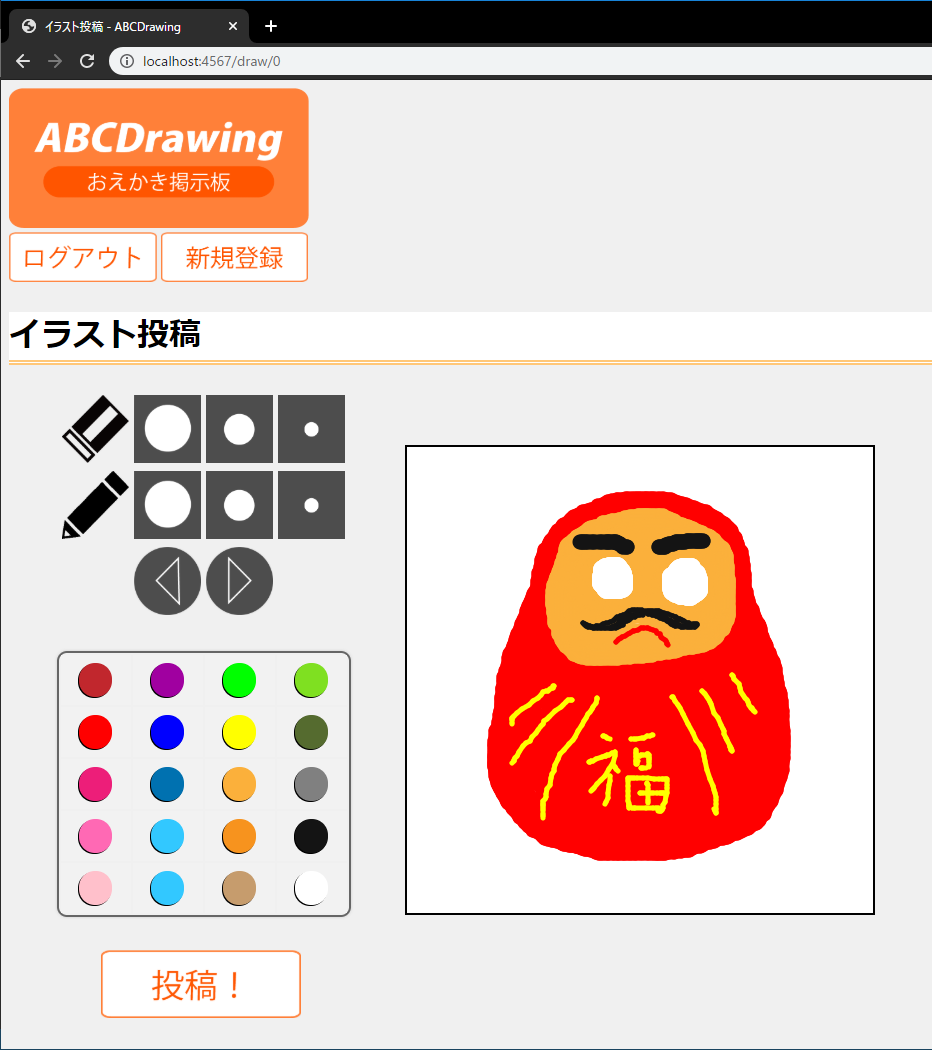
\includegraphics[width=14cm]{drawdaruma.png}
  \caption{イラストを描いた様子}
  \label{drawdaruma}
\end{figure}

\begin{figure}[H]
  \centering
  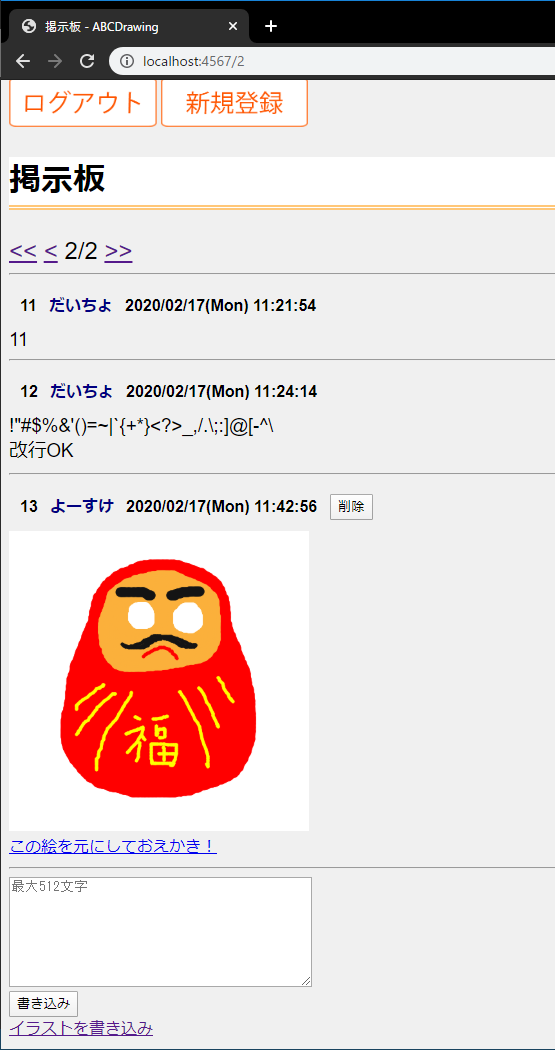
\includegraphics[width=10cm]{drawpost.png}
  \caption{イラストの投稿}
  \label{drawpost}
\end{figure}

\subsection{おえかき}
おえかきの処理は、リスト\ref{drawjs}のdraw.jsで行っている。

canvas上に線を引く関数\texttt{drawLine}は、142行目から定義されている。
canvasのメソッドである\texttt{strokeStyle}, \texttt{lineWidth}で先の色と太さを指定した後、
\texttt{lineTo}で直前のマウス座標から現在のマウス座標に向かって線を引く。
\texttt{drawLine}関数を、マウスが動く度に呼び出されるイベントリスナー内で呼び出すことで、イラストが描ける。

操作履歴を管理するクラス\texttt{History}は、32行目から定義されている。
\texttt{push}メソッドを実行すると、現在のcanvasの状態がそのまま\texttt{log}というリストに記録される。
\texttt{undo}メソッドを実行すると、最新から1つ前の状態のcanvasを\texttt{log}から取得し、\texttt{return}する。\texttt{redo}メソッドはその逆である。

投稿ボタンが押されると、198行目の\texttt{post}関数が呼び出される。
描いたイラストをBase64でエンコードしたURLに変換し、それをサーバーにPOSTし、データベースに登録することで投稿する。

\subsection{他人の絵を元にしたイラスト投稿}
1から自分でイラストを描く以外に、他人が描いたイラストを元にして追加で描き込める機能を実装した。
図\ref{drawpost}の投稿にある、``この絵を元にしておえかき''というリンクをクリックすると、図\ref{origin}のようにそのイラストの上から描き込むことができる。
この状態で投稿ボタンを押したときの様子を図\ref{originpost}に示す。
図\ref{originpost}を見ると、元にした投稿へのリンクと共にイラストが投稿されているのが分かる。

\begin{figure}[H]
  \centering
  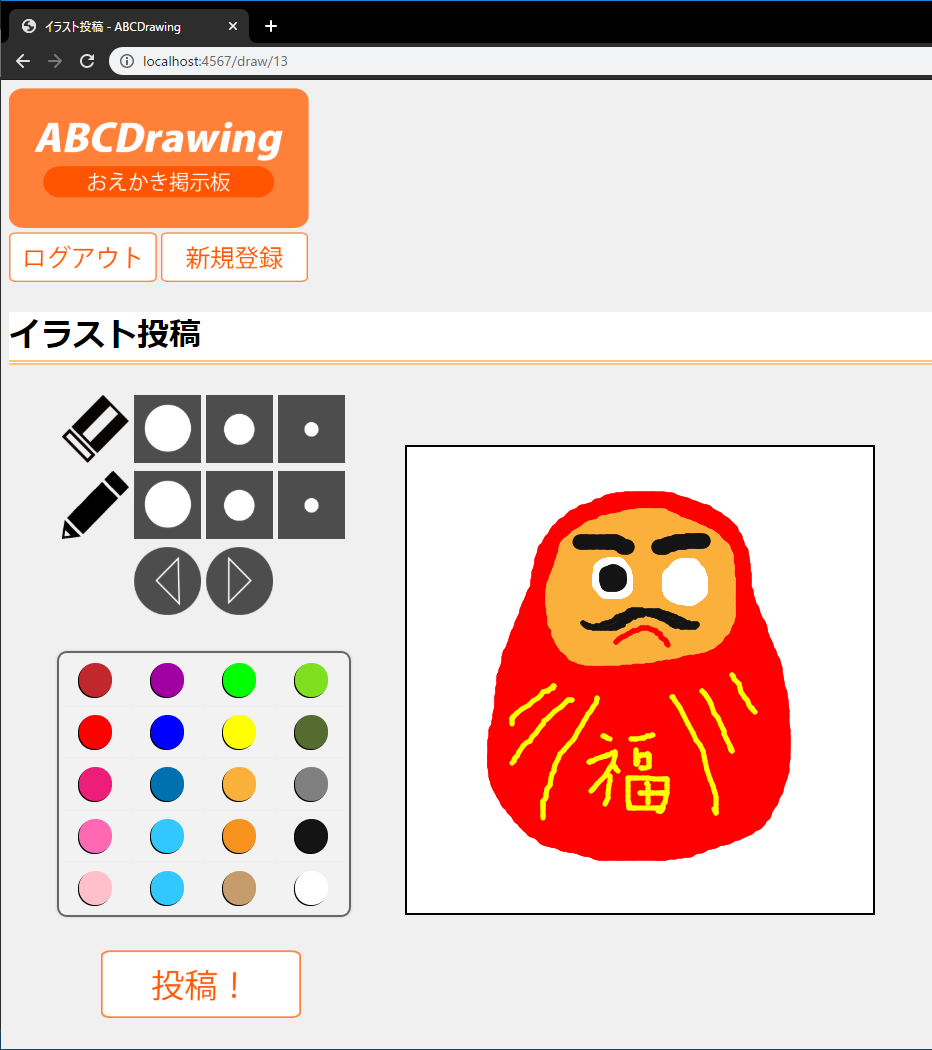
\includegraphics[width=14cm]{origindraw.png}
  \caption{他人の絵を元にイラストを描く様子}
  \label{origin}
\end{figure}

\begin{figure}[H]
  \centering
  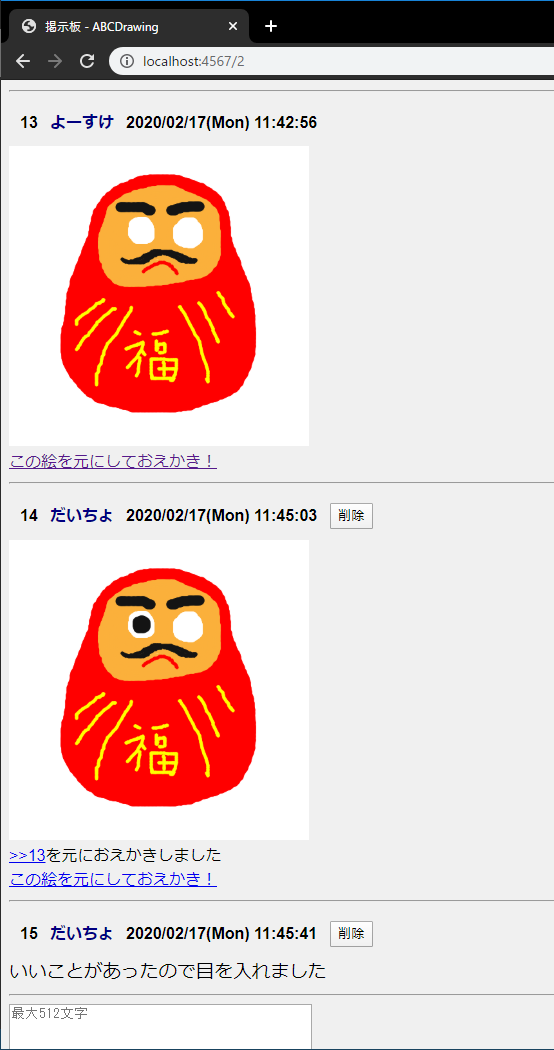
\includegraphics[width=10cm]{originpost.png}
  \caption{他人の絵を元にイラストを投稿した様子}
  \label{originpost}
\end{figure}

\subsection{ページ切り替え}
10件以上の投稿がある場合には、2ページ以降が追加される機能を実装した。
図\ref{f5}のように、すでに10件の投稿がある状態で投稿をすると2ページ目に投稿が追加される。
投稿された後の状態を図\ref{f6}に示す。
図\ref{f6}を見ると、新たに2ページ目が追加され、そこにリダイレクトされていることが分かる。

\begin{figure}[H]
  \centering
  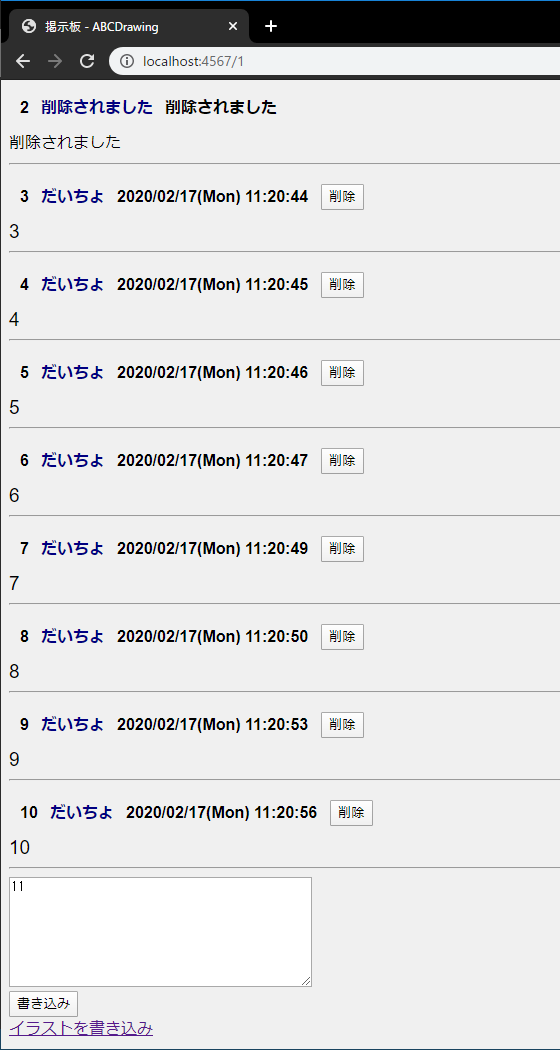
\includegraphics[width=10cm]{bbs07.png}
  \caption{10件の投稿がある状態}
  \label{f5}
\end{figure}

\begin{figure}[H]
  \centering
  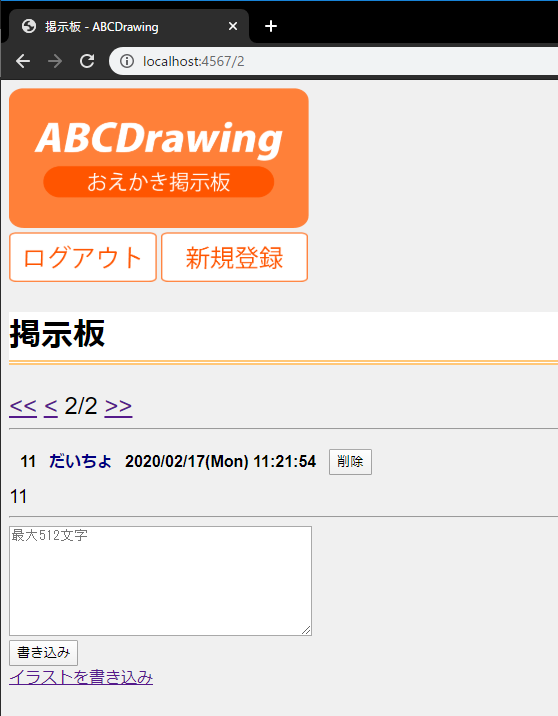
\includegraphics[width=10cm]{bbs08.png}
  \caption{11件目の投稿}
  \label{f6}
\end{figure}

ページ番号はURLに指定できる。
指定されたページ番号ををbbs.rbの223行目で受け取り、そのページに相当する投稿を表示する。
なお、範囲外のURLが入力された場合は、エラーページを表示する。
エラーページが表示された様子を図\ref{f7}に示す。

\begin{figure}[H]
  \centering
  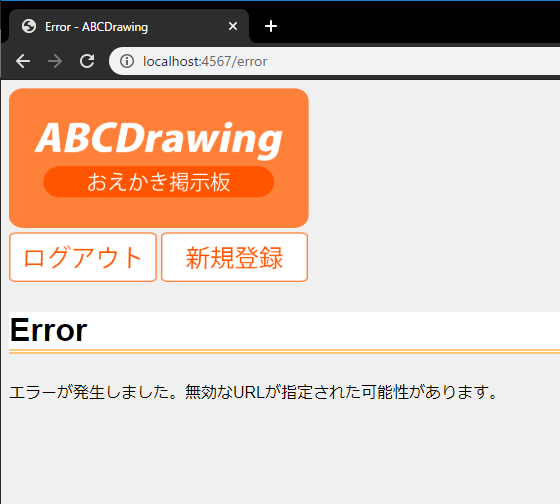
\includegraphics[width=10cm]{bbs11.png}
  \caption{エラーページ}
  \label{f7}
\end{figure}

\subsection{CSSの設定}
ページを見やすくするために、CSSを設定した。
全てのページで共通するスタイルはリスト\ref{commoncss}のcommon.cssで指定し, 各ページのみで適用させたいスタイルは別途指定するような仕様にすることで、メンテナンス性を向上させた。

CSSを設定していないページを図\ref{f8}に示す。
CSSを設定することで色合いや間隔などを調整することで見やすくなることが分かる。

\begin{figure}[H]
  \centering
  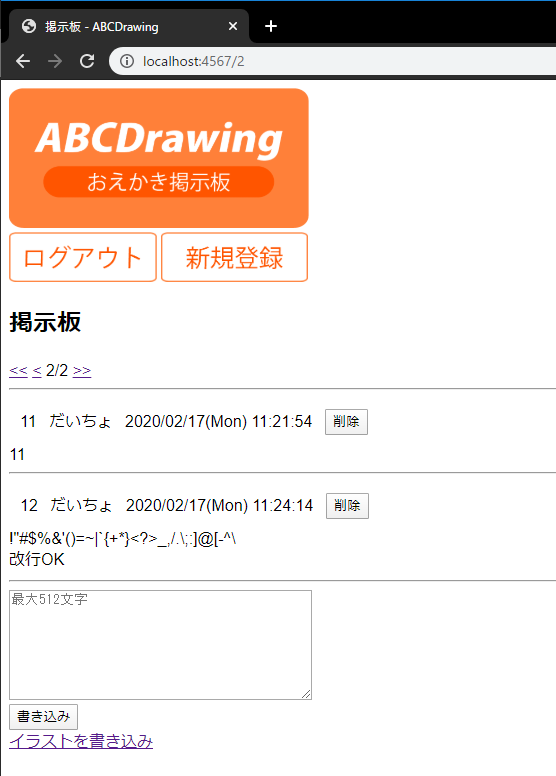
\includegraphics[width=10cm]{bbs12.png}
  \caption{CSSを設定していないページ}
  \label{f8}
\end{figure}


\end{document}
